\item \textbf{{[}RVHS/PRELIM/9569/2021/P1/Q4{]} }

Answer all questions. 
\begin{center}
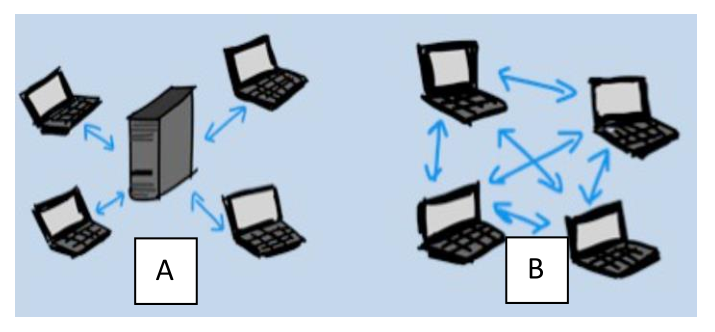
\includegraphics[width=0.5\paperwidth]{C:/Users/Admin/Desktop/Github/question_bank/LyX/static/img/9569-RVHS-2021-P1-Q4}
\par\end{center}
\begin{enumerate}
\item State the network architecture model of A and B as shown in the diagram
below.\hfill{} {[}1{]}
\item State an advantage of model A over B in the diagram above.\hfill{}{[}1{]}
\item State and explain if each of the following statements are correct.
\hfill{}{[}6{]}
\begin{itemize}
\item \textquotedblleft One of the functionalities of the DNS is that different
users can simultaneously receive different IP translations for the
same domain name.\textquotedblright{} 
\item \textquotedblleft The 4 top layers of TCP/IP model are application,
internet, data link and physical.\textquotedblright{} 
\item \textquotedblleft The internet layer is not responsible for reliable
transmission. It makes no guarantees about the proper arrival of packets.\textquotedblright{} 
\item \textquotedblleft 2C:54:91:G8:F9:E3 is a valid MAC address.\textquotedblright{} 
\item \textquotedblleft 2001:0db8:0001:0ab9:C0A8:0102 is a valid IPv6 address.\textquotedblright{} 
\item \textquotedblleft The internet and the World Wide Web are the same
thing.\textquotedblright{} 
\end{itemize}
\item State the purpose of HTTP and explain how the protocol works. \hfill{}{[}3{]}
\item Explain packet switching. \hfill{}{[}1{]}
\item State an ethical issue related to artificial intelligence.\hfill{}
{[}1{]}
\item State the purpose of defining the code of conduct for computer use.
\hfill{}{[}2{]}
\item State a difference between data validation and data verification.\hfill{}
{[}1{]}
\end{enumerate}